\documentclass{standalone}
\usepackage{tikz}
\usetikzlibrary{positioning, arrows.meta, shapes, fit}

\begin{document}

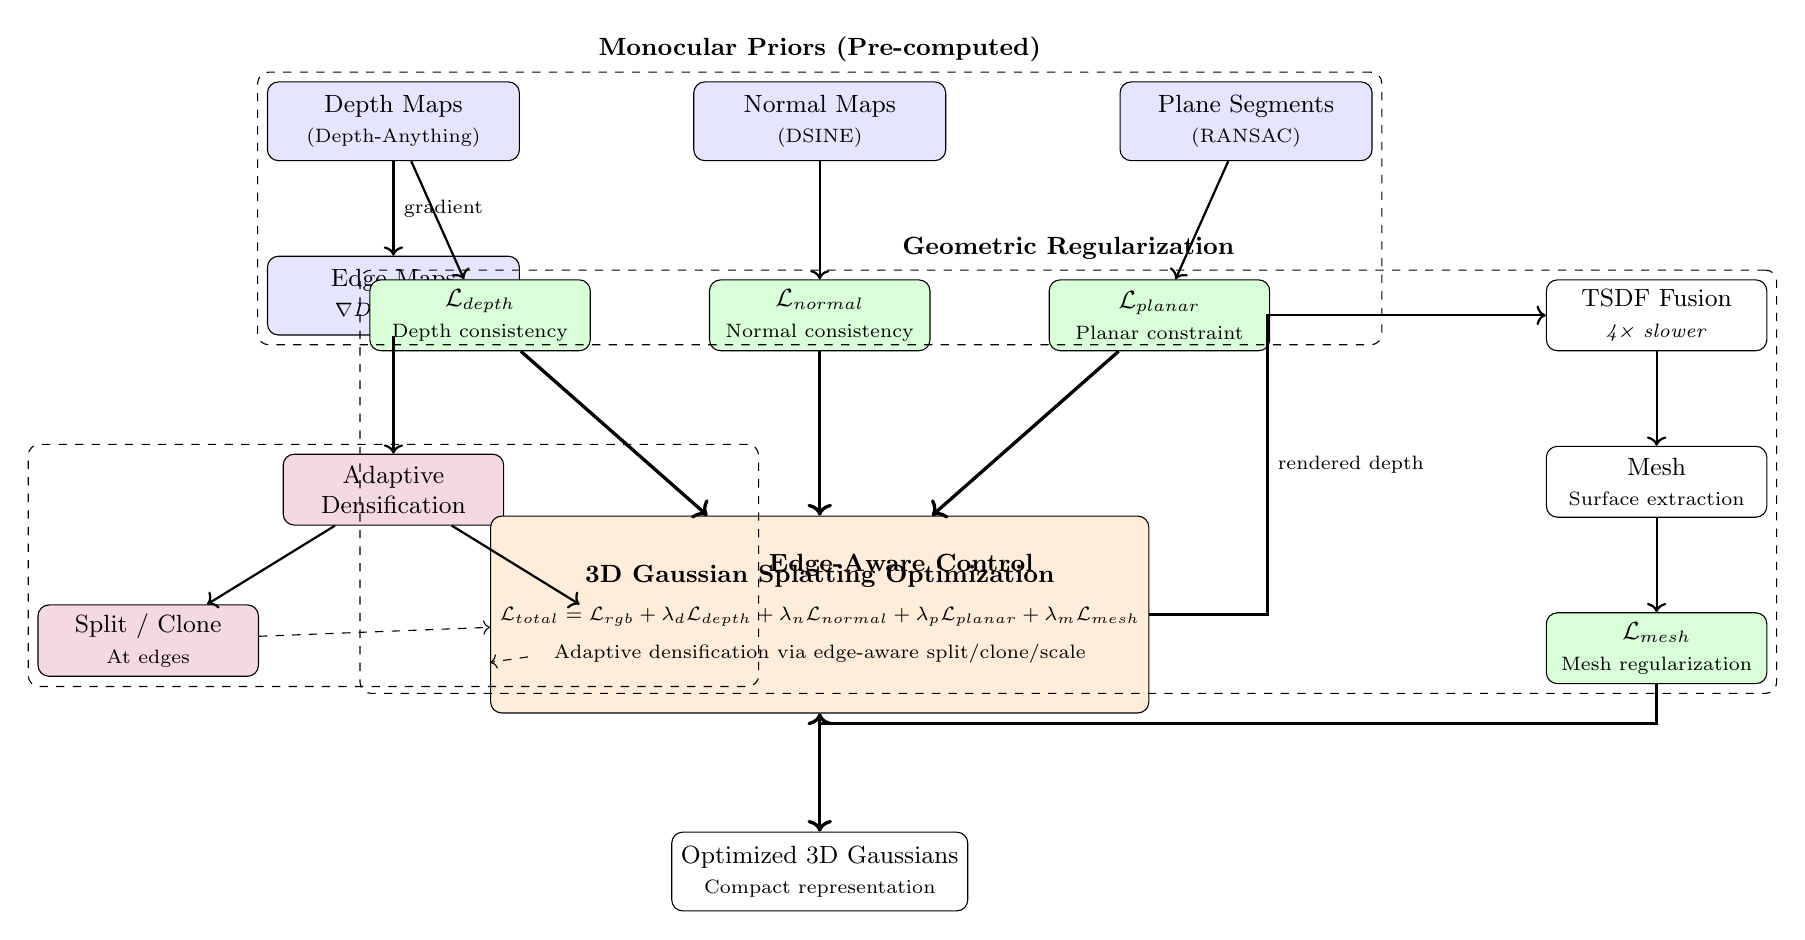
\begin{tikzpicture}[
    font=\small,
    node distance=1.8cm and 2.2cm,
    box/.style={draw, rounded corners, minimum width=3.2cm, minimum height=1cm, align=center},
    smallbox/.style={draw, rounded corners, minimum width=2.8cm, minimum height=0.9cm, align=center},
    arrow/.style={->, thick},
    mainarrow/.style={->, very thick},
    dashedarrow/.style={->, dashed}
]

% =====================
% INPUT PRIORS (TOP)
% =====================
\node[box, fill=blue!10] (depth) {Depth Maps\\{\scriptsize (Depth-Anything)}};
\node[box, fill=blue!10, right=of depth] (normal) {Normal Maps\\{\scriptsize (DSINE)}};
\node[box, fill=blue!10, right=of normal] (plane) {Plane Segments\\{\scriptsize (RANSAC)}};

\node[box, fill=blue!10, below=1.2cm of depth] (edge) {Edge Maps\\{\scriptsize $\nabla D > \tau_{edge}$}};

% =====================
% LOSSES (MIDDLE)
% =====================
\node[smallbox, fill=green!15, below=1.5cm of depth, xshift=1.1cm] (ldepth) {$\mathcal{L}_{depth}$\\{\scriptsize Depth consistency}};
\node[smallbox, fill=green!15, below=1.5cm of normal] (lnormal) {$\mathcal{L}_{normal}$\\{\scriptsize Normal consistency}};
\node[smallbox, fill=green!15, below=1.5cm of plane, xshift=-1.1cm] (lplanar) {$\mathcal{L}_{planar}$\\{\scriptsize Planar constraint}};

% =====================
% MESH BRANCH
% =====================
\node[smallbox, right=3.5cm of lplanar] (tsdf) {TSDF Fusion\\{\scriptsize \textit{4× slower}}};
\node[smallbox, below=1.2cm of tsdf] (mesh) {Mesh\\{\scriptsize Surface extraction}};
\node[smallbox, below=1.2cm of mesh, fill=green!15] (lmesh) {$\mathcal{L}_{mesh}$\\{\scriptsize Mesh regularization}};

% =====================
% EDGE-AWARE BRANCH
% =====================
\node[smallbox, fill=purple!15, below=1.5cm of edge] (densify) {Adaptive\\Densification};
\node[smallbox, fill=purple!15, below left=1cm and 0.3cm of densify] (split) {Split / Clone\\{\scriptsize At edges}};
\node[smallbox, fill=purple!15, below right=1cm and 0.3cm of densify] (scale) {Gaussian Scaling\\{\scriptsize $s_{edge} < s_{planar}$}};

% =====================
% OPTIMIZATION (BOTTOM)
% =====================
\node[box, fill=orange!15, below=4.5cm of normal, minimum width=7cm, minimum height=2.5cm] (opt) {
\textbf{3D Gaussian Splatting Optimization}\\[0.3em]
{\scriptsize $\mathcal{L}_{total} = \mathcal{L}_{rgb} + \lambda_d \mathcal{L}_{depth} + \lambda_n \mathcal{L}_{normal} + \lambda_p \mathcal{L}_{planar} + \lambda_m \mathcal{L}_{mesh}$}\\[0.3em]
{\scriptsize Adaptive densification via edge-aware split/clone/scale}
};

\node[box, below=1.5cm of opt] (output) {Optimized 3D Gaussians\\{\scriptsize Compact representation}};

% =====================
% CONNECTIONS
% =====================

% Priors → losses
\draw[arrow] (depth) -- (ldepth);
\draw[arrow] (normal) -- (lnormal);
\draw[arrow] (plane) -- (lplanar);

% Depth → edge
\draw[arrow] (depth) -- node[right, font=\scriptsize] {gradient} (edge);

% Edge → densification
\draw[arrow] (edge) -- (densify);
\draw[arrow] (densify) -- (split);
\draw[arrow] (densify) -- (scale);

% Mesh branch (from optimization rendered depth)
\draw[arrow] (opt.east) -- ++(1.5,0) |- node[near start, right, font=\scriptsize] {rendered depth} (tsdf);
\draw[arrow] (tsdf) -- (mesh);
\draw[arrow] (mesh) -- (lmesh);

% Losses → optimization
\draw[mainarrow] (ldepth) -- (opt);
\draw[mainarrow] (lnormal) -- (opt);
\draw[mainarrow] (lplanar) -- (opt);
\draw[mainarrow] (lmesh.south) -- ++(0,-0.5) -| (opt.south);

% Edge-aware affects optimization
\draw[dashedarrow] (split) -- (opt);
\draw[dashedarrow] (scale) -- (opt);

% Optimization → output
\draw[mainarrow] (opt) -- (output);

% =====================
% GROUP BOXES (VISUAL STRUCTURE)
% =====================
\node[draw, dashed, rounded corners, fit=(depth)(normal)(plane)(edge), label=above:{\textbf{Monocular Priors (Pre-computed)}}] {};
\node[draw, dashed, rounded corners, fit=(ldepth)(lnormal)(lplanar)(lmesh), label=above:{\textbf{Geometric Regularization}}] {};
\node[draw, dashed, rounded corners, fit=(densify)(split)(scale), label=right:{\textbf{Edge-Aware Control}}] {};

\end{tikzpicture}

\end{document}
